\chapter{Guest Speaker Maurice ``Hank'' Greenberg}

This lecture is unusual in form and central in substance. Robert J. Shiller presents Maurice ``Hank'' Greenberg not as a decorative guest, but as a case study in how finance actually lives inside institutions: in underwriting, incentives, capital structure, product design, regulation, and the governance of risk. The mathematics is therefore not blackboard mathematics. It appears instead as a disciplined way of organizing claims about insurance, diversification, leverage, liquidity, and the contractual mechanics that turned a large balance sheet into a fragile one.

\section{Finance Beyond Formulas}

Shiller opens by telling us how to listen. The course is interested in finance, but not in finance understood only as formal asset-pricing or CAPM-style modeling. It is also interested in how institutions are financed, how people are chosen and motivated, and how character and judgment enter into economic life. That frame matters because Greenberg's lecture begins with biography and business history, yet it never leaves the domain of finance.

Greenberg begins with war, law school, and contingency. He enlisted in the Army before finishing high school, served in Europe during World War II, returned to finish school, went on to law school, and then found himself after Korea with a degree, a family, and the immediate problem of finding work. In the lecture this is not merely autobiographical scene setting. It establishes the background from which his view of risk emerges: one enters finance not first through formulas, but through decisions under uncertainty, institutional discipline, and responsibility.

That is why the first true analytical turn comes only when he arrives in insurance. The lecture does not begin by defining insurance abstractly. It begins by showing how someone ended up inside an insurance company and then had to learn what the business was really about.

\section{From Soldier to Underwriter}

Greenberg's entry into insurance is almost accidental. He returns from Korea, decides he does not want to practice law, walks into an insurance company, and eventually starts as a junior underwriter. At that point the lecture stops moving by anecdote and begins moving by definition.

\begin{definition}
An underwriter studies a proposed risk and decides whether the firm should write it. In a more formal rendering, if risk \(i\) would generate underwriting profit \(\pi_i\) under the available information set \(\mathcal{I}\), then the firm writes the contract only if the expected result is acceptable:
\begin{equation}
\text{write risk } i \quad \text{only if} \quad \mathbb{E}[\pi_i \mid \mathcal{I}] > 0.
\end{equation}
\end{definition}

\begin{remark}
This inequality is a cautious reconstruction of Greenberg's verbal definition. It is not a board equation from the lecture. Its purpose is to make explicit what his description already implies: underwriting is an acceptance rule under uncertainty.
\end{remark}

The special risk division in which he worked gives content to the rule. Different days bring different risks: sports events, accidental-death coverage for executives, and other unusual exposures. The essential point is that underwriting is not a mechanical filing operation. One has to inspect the structure of the risk, decide whether the premium compensates for it, and determine whether the firm wants that exposure on its books.

\subsection{Question \& Answer}

Why is underwriting the first mathematical core of the lecture?

Because it is the first place where Greenberg turns biography into mechanism. Once we say that the insurer examines a risk and decides whether to write it, the rest of the lecture can be read as the scaling-up of this same logic. A turnaround, an acquisition, a reinsurance treaty, a diversification strategy, even a refusal to enter a corrupt market, are all variations on the same question: which risks do we accept, on what terms, and with what protections?

\section{Turning Around American Home and Building AIG}

The lecture next moves from individual underwriting to institutional underwriting. Greenberg meets C.\ V.\ Starr, joins Starr's organization, and is sent to American Home, a company that is old, well known, and failing. The reason for failure, as Greenberg tells it, is not mysterious. American Home writes business through agents, but the agency organization is weak, so the quality of the business is poor and the company loses money year after year.

Here again the lecture is organized by diagnosis first and remedy second. The problem is not simply that losses are high. The problem is that the distribution structure itself selects the wrong business. Greenberg's answer is to remove the agents, move into the brokerage business, and begin writing larger commercial risks. That decision changes the scale of the game. Once one writes large property, casualty, marine, and aviation risks, one also needs reinsurance and needs it on credible terms. Hence the move to London and Lloyd's.

The institutional logic is straightforward. Better underwriting requires better people; large risks require reinsurance support; rapid success creates a capital bottleneck; and capital bottlenecks push the firm toward acquisition and holding-company structure. In the lecture the sequence is very clear: fix the underwriting model, build a strong underwriting group, solve the reinsurance problem, then solve the capital problem.

By the mid-1960s that logic produces the next structural step. National Union and then New Hampshire are acquired, their business models are repaired in essentially the same way, and in 1967 AIG is created as the holding company over these entities. The chapter should preserve this rhythm. AIG is not introduced as a name first and a structure second. It is introduced as the outcome of a series of operational solutions.

\section{Innovation, Diversification, and Open Markets}

Once the core business is repaired, Greenberg turns to the conditions of scale. The lecture names several of them: product innovation, diversification, expense discipline, and access to markets that are not naturally open to foreign insurers. These do not appear as separate themes. They are one operating philosophy viewed from different angles.

The product side is concrete. AIG introduces directors and officers liability insurance, political risk insurance, and kidnap and ransom insurance. These examples matter because they show how insurance grows by identifying needs that are not yet fully served. AIG's distinctiveness, in Greenberg's account, lies not merely in writing insurance efficiently, but in inventing insurable forms where business demand already exists.

The diversification argument is the first place where the lecture invites a clean mathematical restatement.

\begin{proposition}
If the insurer's aggregate outcome is
\begin{equation}
X = \sum_{j=1}^{n} X_j,
\end{equation}
where each \(X_j\) is the profit or loss from a line of business or geography, then imperfect correlation across the \(X_j\) reduces the volatility of the aggregate result relative to a naive sum of stand-alone volatilities.
\end{proposition}

\begin{proof}
We expand the variance:
\begin{equation}
\operatorname{Var}(X)
=
\sum_{j=1}^{n}\operatorname{Var}(X_j)
+
2\sum_{j<k}\operatorname{Cov}(X_j,X_k).
\end{equation}
If the covariances are not all maximally positive, then diversification prevents aggregate variance from rising one-for-one with the sum of stand-alone variances. This is the mathematical content of Greenberg's claim that broader diversification provides greater stability.
\end{proof}

Greenberg does not write that variance expansion on the board, but his verbal claim is unmistakable: property-casualty insurance is volatile because earthquakes, hurricanes, and changing economic environments strike unevenly, and geographic as well as product diversification stabilizes the firm.

\subsection{Question \& Answer}

Why does diversification stabilize an insurance company?

Because the firm's losses do not all arrive from the same source at the same time. If country, product, and event risks are not perfectly synchronized, then the aggregate result fluctuates less violently than any one concentrated book of business. In lecture language, more diversification gives greater stability. In formal language, the covariance terms do the work.

Greenberg also gives a second numerical expression of operating discipline. He says that many insurers run expense ratios around \(30\%\), whereas AIG ran at approximately \(19\%\):
\begin{equation}
\mathrm{ER}_{\text{industry}} \approx 30\%,
\qquad
\mathrm{ER}_{\text{AIG}} \approx 19\%.
\end{equation}
Again the lecture's style is to state the number and then interpret it institutionally. The lower ratio comes not from a single trick, but from efficiency, better execution, and proper use of reinsurance.

Diversification then opens outward into geopolitics. Greenberg explains that in order to diversify internationally one must first open markets, and many such markets did not want to be opened. Japan is the emblematic case in the lecture, but China becomes the longer strategic example. The numerical chronology is worth preserving:
\begin{equation}
1975 \longrightarrow 1992.
\end{equation}
That is the span Greenberg gives from his first visit to China to the granting of the first life-insurance license to a foreign company. He also stresses the asymmetry of ownership:
\begin{equation}
\text{typical foreign ownership ceiling} = 49\%,
\qquad
\text{AIG ownership} = 100\%.
\end{equation}

The lecture insists that finance and state power are intertwined here. Market access required trade negotiations, foreign-policy attention, and a willingness to use government leverage when foreign governments kept their markets closed. It also required a line the firm would not cross: Greenberg emphasizes the refusal to bribe. That point belongs in the chapter because it shows that institutional discipline and risk discipline are not separable.

\section{Organization, Incentives, and the Internal Logic of AIG}

Having described how AIG grows outward, Greenberg turns inward and asks how a company becomes coordinated enough to sustain such growth. The answer is not one thing but a package: culture, mobility, compensation, ownership, and a management group that in his words functioned like a band of brothers.

The MOP system is central in that story. ``Mobile Overseas'' means that a manager may be in one country now and another six months later. The category is not merely administrative; it is prestigious. One has to earn it. The underlying idea is that an international insurer cannot act like a federation of local satrapies. It needs a cadre that treats the whole organization as its field of operation.

The compensation story is equally structural. Greenberg says that nobody could earn more than one million dollars in salary, and that the firm targeted roughly \(15\%\) annual growth:
\begin{equation}
g \approx 15\% \text{ per year},
\qquad
\text{salary} \le 1\text{ million dollars}.
\end{equation}
That salary cap is not anti-compensation; it is a reallocation of compensation. Pay is moved away from fixed salary and toward performance-linked reward, especially deferred equity.

He also gives a compact ownership history. The private Starr entities initially own all of AIG, but rapid growth requires new capital, so ownership becomes diluted even while the company becomes vastly more valuable:
\begin{equation}
\text{initial control of AIG} = 100\%,
\qquad
\text{later control} \approx 15\%.
\end{equation}
\begin{equation}
\text{market capitalization}: 300\text{ million dollars} \to 200\text{ billion dollars}.
\end{equation}
The mathematical point is simple but important. A smaller share of a much larger enterprise may represent much greater economic power than complete ownership of a small one. Growth and dilution are not opposites here; they are linked.

The deferred-equity mechanism is perhaps the cleanest institutional design in the lecture. If goals are met over a two-year horizon, shares are set aside for retirement:
\begin{equation}
\text{goals met over two years}
\Rightarrow
\text{deferred AIG shares at retirement}.
\end{equation}
Leaving early means walking away from those shares. This is Greenberg's version of golden handcuffs.

\subsection{Question \& Answer}

If top managers have no long-term contracts, what keeps them aligned with the firm?

Greenberg's answer has two layers. The first is cultural: one stays because one believes in the company and wants to build it. The second is financial: performance bonuses and deferred stock make success inside the firm much more valuable than exit. A contract forces legal retention; this structure aims at economic and organizational retention.

The lecture closes this section with a deep managerial claim that returns in the final Q\&A: culture starts at the top. The chief executive is not outside risk management. He is the top risk manager. That statement does a great deal of work in the chapter, because it binds governance, incentives, and risk into one theory of the firm.

\section{AIG Financial Products and the Mechanism of Crisis}

The narrative now breaks sharply. Greenberg has just described a vast, profitable, diversified insurer with strong internal controls. Then he asks: what happened?

Before the crisis mechanism itself, the lecture inserts one more layer of institutional setup. AIG expands into life insurance, consumer finance, and related financial services. It creates AIG Financial Products. In Greenberg's telling this unit is initially successful, staffed by mathematically sophisticated people, fully hedged, and monitored through mirrored computer systems as well as enterprise-wide risk management. He is explicit that the company monitored market risk and credit risk throughout the organization. He is also explicit that the weekly discipline of monitoring mattered. After his departure, the key meetings on real-time management, hedging, and risk management were discontinued. The lecture wants us to hear this not as an anecdotal complaint, but as a causal weakening of the control structure.

\begin{definition}
We shall distinguish liquidity from solvency. A firm is solvent if its assets and protected capital are sufficient to meet its obligations in an economic sense. A firm is liquid if it can produce cash quickly enough to meet short-run calls for payment, especially collateral calls.
\end{definition}

The lecture's central mechanism is then presented as a comparison between two contractual regimes for credit default swaps on CDO-related exposures:
\begin{align}
\text{old regime:} \quad & \mathbf{1}_{\{\text{default of underlying}\}}
\Rightarrow
\text{CDS payment},\\
\text{new regime:} \quad & \Delta P_{\mathrm{CDO}} < 0
\Rightarrow
C \uparrow.
\end{align}
Under the original logic, the contract responds when the underlying instrument defaults. Under the later logic, a fall in market value is enough to trigger collateral posting even without realized default.

Greenberg's point is that this is a profound shift. It transforms a loss-recognition rule tied to economic default into a cash-demand rule tied to market marking. We can state the rating trigger schematically as
\begin{equation}
R=\mathrm{AAA}
\Rightarrow
C=0,
\qquad
R<\mathrm{AAA}
\Rightarrow
C>0.
\end{equation}
He says that while AIG carried a triple-A rating it did not have to post collateral, but once that rating disappeared the collateral obligation arrived.

\paragraph{Worked example.}
A simple numerical illustration captures the mechanism Greenberg has in mind. Suppose a reference CDO is carried near par and later marked at \(60\) on a \(100\) scale:
\begin{align}
P_0 &= 100,\\
P_1 &= 60,\\
\Delta P_{\mathrm{CDO}} &= -40.
\end{align}
Under the old default-trigger regime, a temporary mark from \(100\) to \(60\) does not itself require payment if the underlying has not defaulted. Under the later collateral regime, the decline in value can require a collateral posting of roughly \(40\), even though the loss is not yet realized through default. This is an illustrative reconstruction, not a literal reproduction of a contract term from the lecture, but it captures Greenberg's mechanism exactly.

The problem becomes even worse once price discovery fails. Greenberg says there was no exchange on which these CDOs traded, and therefore no common market price. In schematic form:
\begin{equation}
P_{\mathrm{CDO}}^{(1)} \neq P_{\mathrm{CDO}}^{(2)} \neq \cdots \neq P_{\mathrm{CDO}}^{(m)}.
\end{equation}
Different dealers can quote different values. If collateral depends on those values, then the amount that must be posted becomes unstable and contestable. In Greenberg's account Goldman Sachs marked the relevant CDOs at the lowest levels, which intensified the collateral demands on AIG Financial Products.

\begin{figure}[h]
\centering
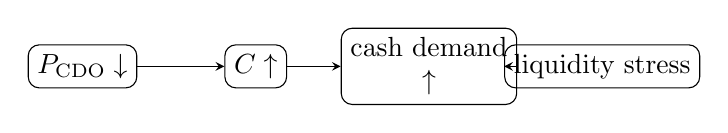
\begin{tikzpicture}[>=stealth, node distance=2.2cm]
\node[draw, rounded corners, align=center] (p) {$P_{\mathrm{CDO}}\downarrow$};
\node[draw, rounded corners, right of=p, align=center] (c) {$C\uparrow$};
\node[draw, rounded corners, right of=c, align=center] (cash) {cash demand\\$\uparrow$};
\node[draw, rounded corners, right of=cash, align=center] (liq) {liquidity stress};
\draw[->] (p) -- (c);
\draw[->] (c) -- (cash);
\draw[->] (cash) -- (liq);
\end{tikzpicture}
\end{figure}

This is the heart of the chapter. The firm can remain economically large, even have solvent regulated insurance subsidiaries, and yet fail on liquidity. Greenberg stresses exactly that point: the insurance companies were protected under state law, policyholders were protected, and the problem was that the parent firm ran out of cash under collateral pressure.

\subsection{Question \& Answer}

How can a firm fail on collateral and cash even if its insurance subsidiaries remain solvent?

Because the collateral mechanism does not wait for slow economic resolution. It demands immediate cash against marked losses. If the firm has to post collateral in massive amounts, and if its rating downgrade activates those obligations, then liquidity can disappear before the underlying assets have actually defaulted. The lecture's distinction between state-regulated insurance capital and parent-level funding pressure is essential here.

The rescue that follows is also described numerically. In Greenberg's account, AIG receives an \(85\) billion dollar Federal Reserve loan at \(14.5\%\) interest, and the government takes \(79.9\%\) of the equity:
\begin{equation}
\text{Fed loan} = 85\text{ billion dollars},
\qquad
r = 14.5\%,
\qquad
\text{equity taken} = 79.9\%.
\end{equation}
He later says government ownership rises to approximately \(92\%\):
\begin{equation}
\text{government ownership of AIG} \approx 92\%.
\end{equation}
He also contrasts this with other rescue arrangements, especially Citigroup:
\begin{equation}
\text{Citigroup support} \approx 30\% \text{ equity},
\qquad
\text{AIG support} \approx 92\% \text{ equity}.
\end{equation}

Here the notes should be careful. These rescue terms are lecture content and should be preserved, but the chapter should present surrounding judgments as Greenberg's own account. In particular, his claim that valuations were effectively in the \(40\) to \(60\) cents-on-the-dollar range, while counterparties were paid at \(100\), belongs to his narrative of the rescue rather than to an independently derived model.

\section{From AIG to the Wider Crisis}

After the firm-level mechanism is established, Greenberg widens the frame. The question is no longer simply why AIG failed. It is why the country placed itself in a position where such failures could become systemic.

The lecture gives a causal chain. First, public policy broadens home ownership without maintaining strict affordability discipline. Mortgages are no longer held in the old way by local banks that know the borrower and keep the risk. Instead they are sold onward, especially through Fannie Mae and Freddie Mac. Second, investment banks lever their capital aggressively:
\begin{equation}
L = \frac{A}{E},
\qquad
L_{\text{investment banks}} \approx 30\times \text{ to } 50\times,
\qquad
L_{\text{older benchmark}} \approx 5\times \text{ to } 7\times.
\end{equation}
Third, those mortgages are packaged into CDOs and sold as if diversification alone guaranteed safety. Fourth, ratings agencies attach triple-A ratings too easily. Fifth, CDS contracts are written on top of those products. Sixth, the trigger structure changes from default to mark-to-value collateral. Seventh, mark-to-market accounting forces further capital compression:
\begin{equation}
V_t^{\text{book/held-to-maturity}}
\longrightarrow
V_t^{\text{market}}.
\end{equation}

The entire chain can be summarized schematically as
\begin{equation}
\text{weaker mortgage discipline}
\Rightarrow
\text{securitization}
\Rightarrow
\text{CDO proliferation}
\Rightarrow
\text{CDS exposure}
\Rightarrow
\text{collateral stress}
\Rightarrow
\text{systemic fragility}.
\end{equation}

Greenberg then turns to policy in a more direct Q\&A style. Some institutions may be too large or too connected to fail without chaos, but such cases should be rare. Government intervention, in his view, should be minimal and even-handed. He is skeptical of ad hoc rescues, skeptical of post-crisis overregulation, and especially insistent that better regulators matter more than simply more regulation.

\subsection{Question \& Answer}

What regulation does Greenberg think would have prevented the CDS collateral spiral?

He gives two answers. First, return CDS to the older logic in which the contract responds to default rather than to a temporary decline in marked value:
\begin{equation}
\text{CDS should trigger on default, not merely on a temporary fall in market value.}
\end{equation}
Second, create exchange trading and price discovery:
\begin{equation}
\text{exchange trading}
\Rightarrow
\text{price discovery}
\Rightarrow
\text{more disciplined collateral and regulation.}
\end{equation}
He adds a third principle in the same spirit: if the instrument functions like insurance, then it should be regulated with reserves like insurance.

The final student questions sharpen several themes that have been present all along. Boards fail when they cease to understand what a company is actually doing. China becomes again an example of insurance growth, with Greenberg emphasizing the introduction of the agency system and commission-based selling. Entrepreneurship remains possible in insurance because new products and new forms of risk constantly appear. And the lecture closes by returning to the point that began it: culture starts at the top, and the CEO is the top risk manager. In that sense the final answer of the lecture is also its first principle.

\section{Summary}

This chapter is a study in finance beyond formal asset pricing yet not beyond mathematical structure. Greenberg begins with underwriting, where a risk is accepted or rejected under uncertainty; scales that logic into reinsurance, acquisitions, diversification, and global market entry; and then describes how incentives and organizational design hold a large insurer together. The crisis portion of the lecture then isolates a precise mechanism: once credit protection responds to marked loss rather than realized default, and once collateral must be posted into a market without reliable price discovery, liquidity can fail long before the slower question of final solvency is resolved.

The lecture therefore leaves us with two linked lessons. First, insurance, banking, and financial engineering are all forms of risk design, and they must be understood contractually as well as institutionally. Second, no mathematical mechanism remains safe when the surrounding governance, incentive system, and discipline of risk monitoring break down.